\chapter{Plots}
\begin{figure}[H]
\centering
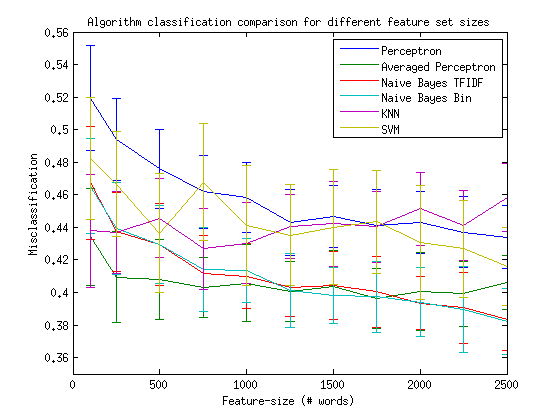
\includegraphics[scale = 1]{../Plottar/feature-size100-2500bigram.png}
\caption{In-domain classification using varying Bigram feature set sizes with 2$\sigma$ height error bars and comparing all algorithms.}
\end{figure} 

\begin{figure}[H]
\centering
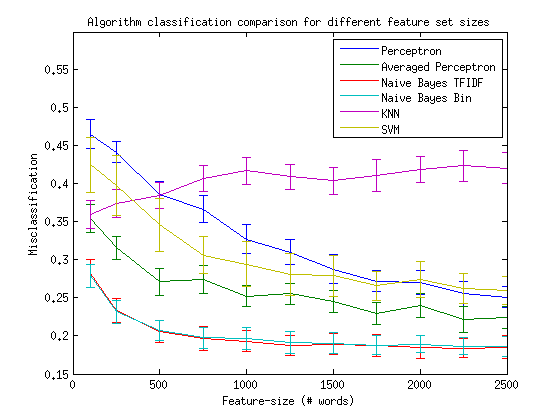
\includegraphics[scale = 1]{../Plottar/feature-size100-2500all.png}
\caption{In-domain sentiment analysis classification error (error bars of height $\sigma$) for the 6 algorithms on varying Unigram feature vector sizes}
\end{figure} 

\begin{figure}[H]
\centering
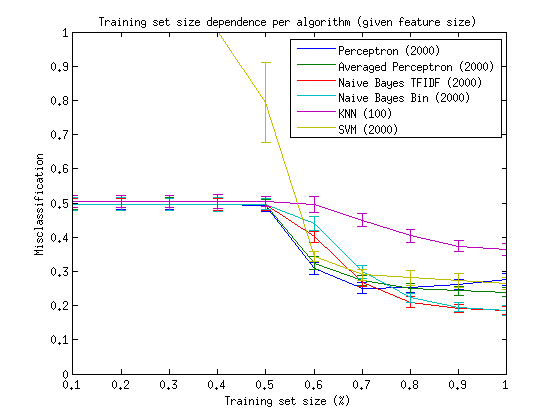
\includegraphics[scale = 1]{../Plottar/training_size_k_2000allknn_100.png}
\caption{In-domain sentiment analysis classification error (error bars of height $\sigma$) for the 6 algorithms on varying training set size $\in \{10\%, 100\%\}$.}
\end{figure} 

\begin{figure}[H]
\centering
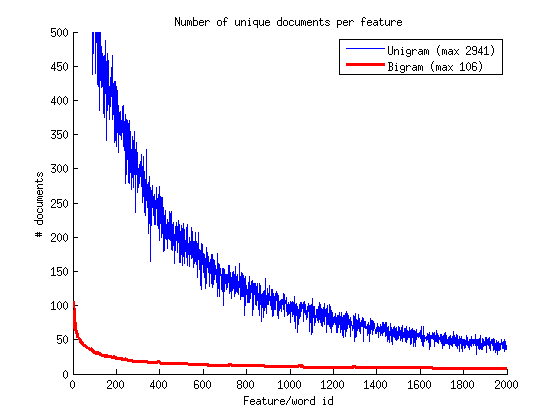
\includegraphics[scale = 1]{../Plottar/documents_per_feature.png}
\caption{Documents per feature}
\end{figure} 

\begin{figure}[H]
\centering
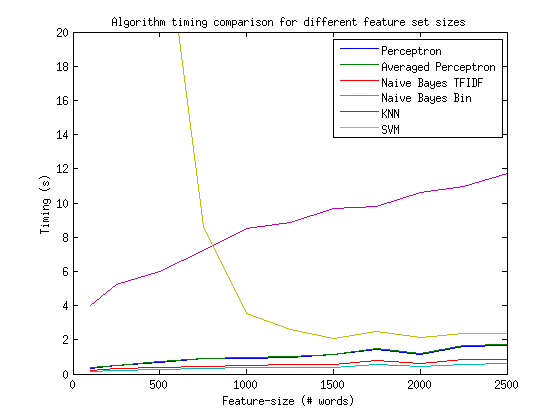
\includegraphics[scale =  1]{../Plottar/feature_size_TIMING.png}
\caption{Running time for different algorithms and feature size}
\end{figure} 

\begin{figure}[H]
\centering
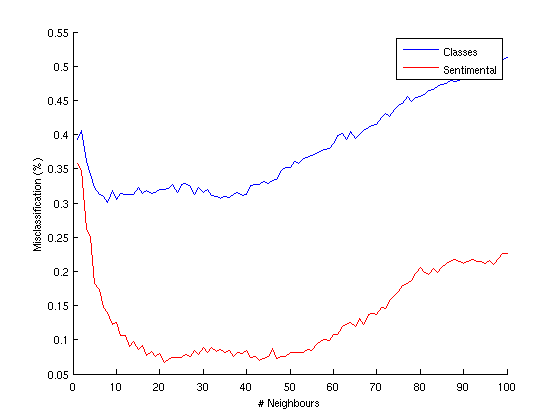
\includegraphics[scale = 1]{../Plottar/knn_2000words_testdata100_unigram.png}
\caption{Plot showing results from the KNN classifier}
\end{figure} 

\begin{sidewaysfigure}[H]
\centering
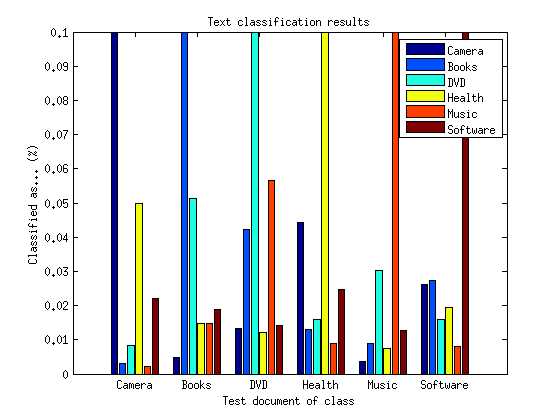
\includegraphics[scale = 0.47]{../Plottar/text_categorization.png}
\caption{The total spread of classifications for the two algorithms Naive Bayes TFIDF and the Averaged Perceptron, showing the fraction of resulting classifications (bars) for each input document of a certain class (x-axis).}
\end{sidewaysfigure} 

\begin{sidewaysfigure}[H]
\centering
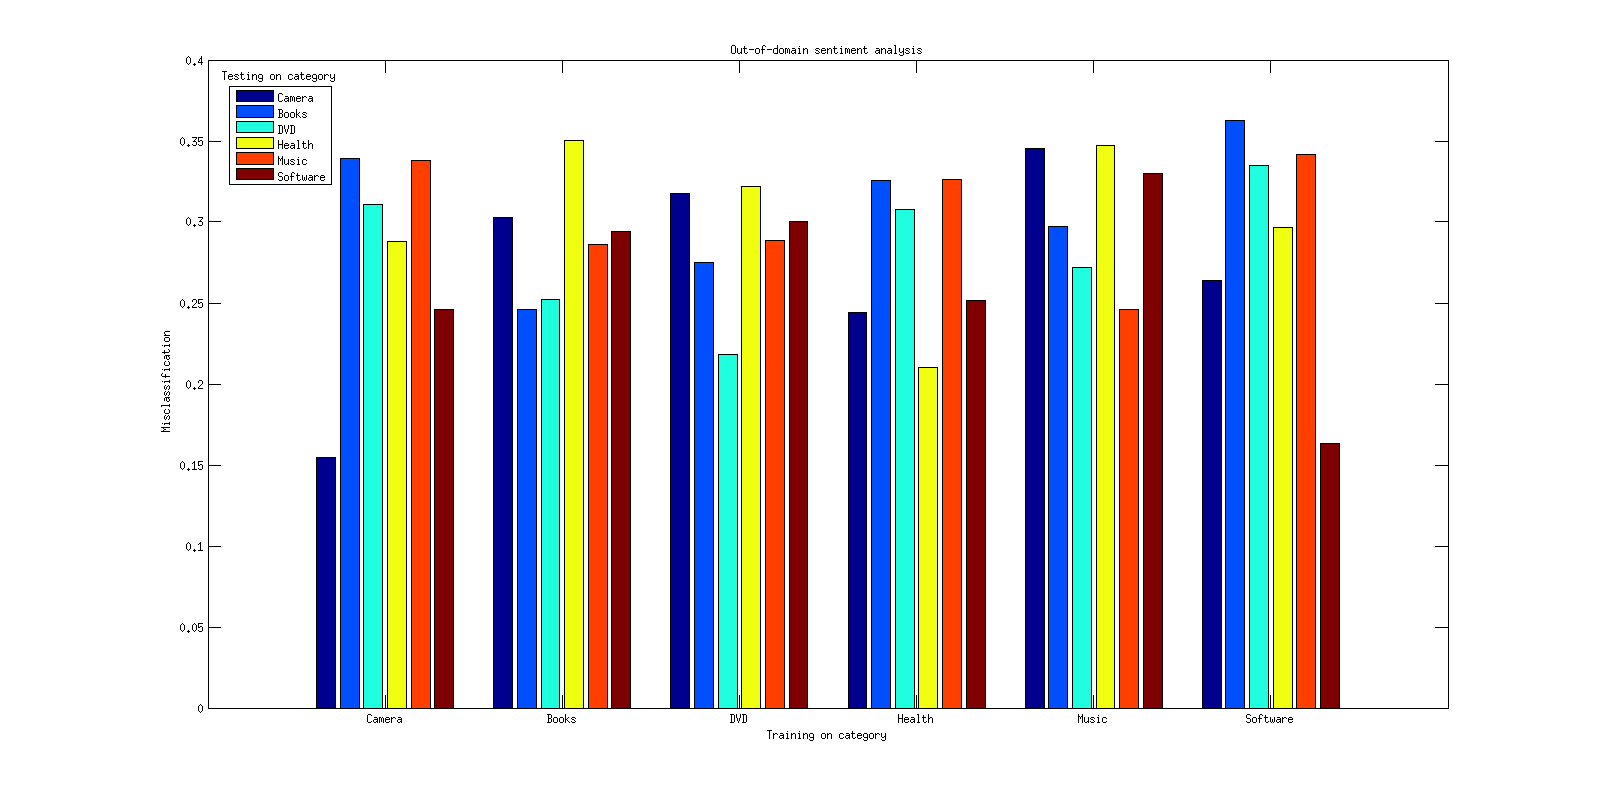
\includegraphics[scale = 0.47]{../Plottar/outofdomain.png}
\caption{The sentiment analysis classification error results of training on a document class subset - represented by a group of bars, and testing on all classes - represented by individual bars.}
\end{sidewaysfigure} 

\begin{figure}[H]
\centering
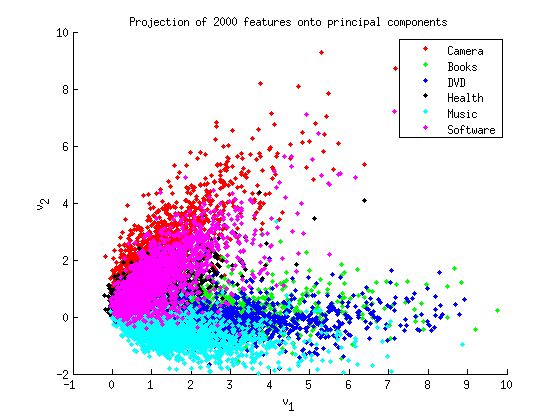
\includegraphics[scale = 1]{../Plottar/pca_all.png}
\caption{Principal Component Analysis showing all categories , (b) DVD and Camera, (c) Health, Software and Camera, (d) Books DVD and Music
}
\end{figure} 

\begin{figure}[H]
\centering
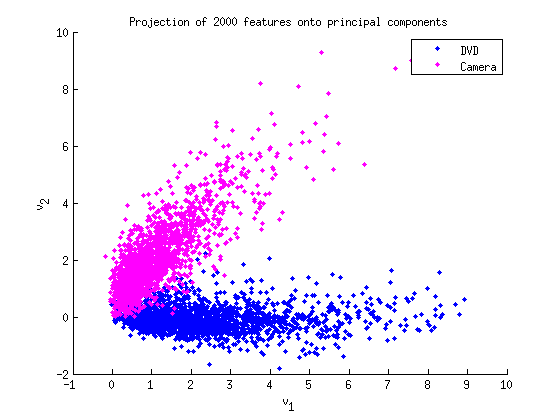
\includegraphics[scale = 1]{../Plottar/pca_nocorr.png}
\caption{Principal Component Analysis showing DVD and Camera}
\end{figure} 

\begin{figure}[H]
\centering
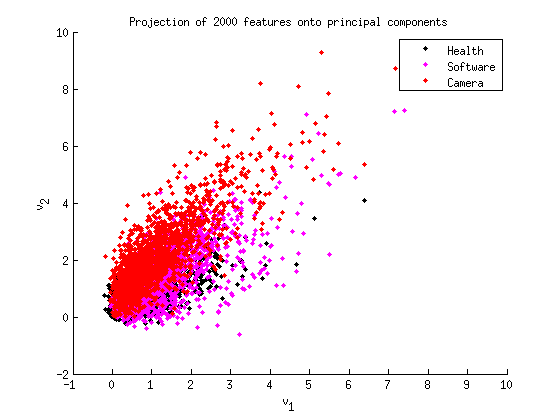
\includegraphics[scale = 1]{../Plottar/pca_largecorr.png}
\caption{Principal Component Analysis showing Health, Software and Camera}
\end{figure} 

\begin{figure}[H]
\centering
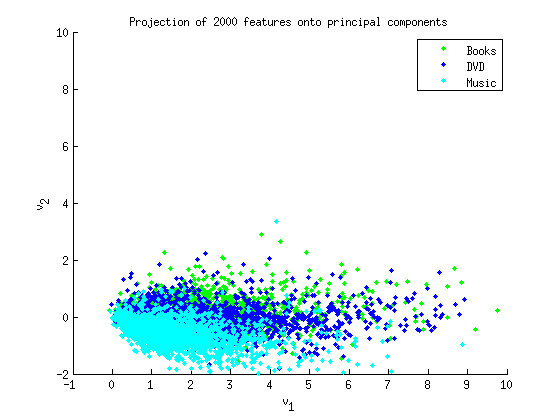
\includegraphics[scale = 1]{../Plottar/pca_somecorr.png}
\caption{Principal Component Analysis showing Books DVD and Music}
\end{figure} 

\begin{figure}[H]
\centering
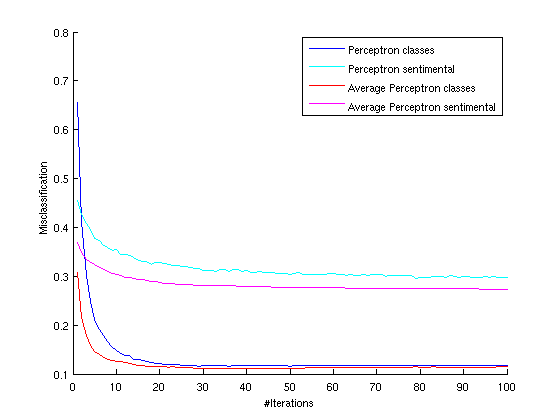
\includegraphics[scale = 1]{../Plottar/perceptron_2000words_unigram_10foldcv_classes-high_sentimental-low.png}
\caption{Plot over misclassifications for different \#iterations}
\end{figure} 

\chapter{Stop-words}
\input{appendix/english_word_stops.txt}
